\fixme{Scattering operator Preisehdorfer}

\fixme{Monte Carlo ray tracing as a chapter}

\chapter{Background}
\label{sec:background}
\begin{itemize}
\item Introduction of relevant theory behind the thesis
\item In photorealistic, introduction to most relevant quantities, namely radiometric quantities, brdfs and bssrdfs. Scattering and non scattering media.
\item Offline and real time techniques. GPUs. 
\item ray tracign and rasterization. bleeding between the two.
\end{itemize}

\section{Photorealistic rendering}

\subsection{Radiometry}
Radiometry is that branch of science that measures electromagnetic radiation. We will define the basic radiometric quantities, in order to then introduce the two main reflectance functions of interest in this thesis, namely the BRDF and the BSSRDF. In particular, we want to give a definition of radiance, the most useful quantity in describing light transport along rays.

First, we consider an ideal point light source in space. The source emits a certain amount of energy $U$, measured in Joules $[J]$. The first quantity we derive is radiant flux or radiant power $\Phi$, defined as the amount of energy per second emitted by the light:
$$
\Phi = \frac{d U}{d t}  \siunit{\watt}.
$$
The radiant flux represents the overall power the light emits in all directions overall. We usually want to be more descriptive on how a light or a surface is emitting light, since not all the sources we consider are ideal. First, we are interested on how the light emission changes  We then define $I$ as radiant intensity, i.e. the amount of flux the light emits towards a specific direction $\vec{\omega}$:
$$
I(\vec{\omega}) = \frac{d \Phi}{d \omega}  \siunit{\watt \per \steradian}.
$$   
Where $d \omega$ is an infinitesimal solid angle around direction $\vec{\omega}$. An isotropic point light, by definition, as constant intensity across all directions.

We now consider a surface that receives light. In particular, we consider an infinitesimal oriented element of this surface $d \vec{A}$ around a point $\mathbf{x}$. The orientation of the surface is usually called the \emph{normal} and indicated by $\vec{n}$ We can now define irradiance as the amount of incoming flux received per unit area:
$$
E(\mathbf{x}) = \frac{d \Phi}{d A}  \siunit{\watt \per \square \metre}
$$
Similarly, we have a dual quantity for the flux \emph{emitted} by a unit element surface. We call this quantity \emph{radiosity} and we define it with the symbol $B$.
The most simple irradiance is the one emitted by an isotropic point light. In this case, the irradiance at a distance $R$ from the point light is 
$$
E = \frac{\Phi}{4 \pi R} \siunit{\watt \per \square \metre}
$$
So, the father we go from a point light, the less irradiance we receive, because the power $\Phi$ has to spread across a larger area.

Finally, we combine the definitions above into one, to define the last important basic radiometric quantity, \emph{radiance}:
$$
L(\mathbf{x}, \vec{\omega}) = \frac{d^2 \Phi}{d A \cos\theta d \omega}  \siunit{\watt \per \square \metre \per \steradian}
$$
Where $\cos \theta = \vec{n} \cdot \vec{\omega}$ is the cosine of the angle between the normal and the direction of evaluation. $d A \cos\theta$ is also called the \emph{projected area element}. As irradiance, radiance can be incoming or outgoing from a specific point. We indicate these quantities with $L_i$ and $L_o$, respectively. In graphics, radiance is usually the most useful quantity for two main reasons. First, the other quantities can be easily computed from radiance through radiometric integrals:
\begin{figure}
\centering
	 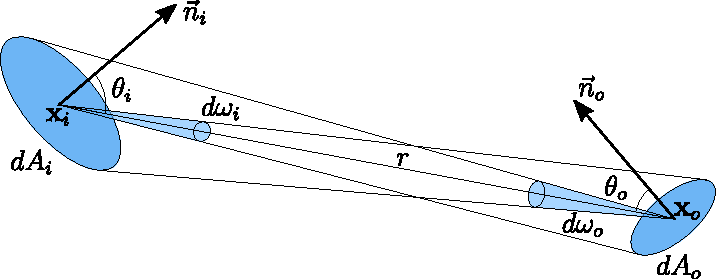
\includegraphics[scale=0.8]{figures/etendue}  \\
\caption{Configuration to prove the equality of radiance across a ray.} %The red rectangle shows where we estimated RMSE in Table \ref{table:quant}.}
\label{fig:etendue}
\end{figure}
\begin{equation*}
\begin{split}
\Phi &= \int_{\Omega} \int_{A} L(\mathbf{x}, \vec{\omega})  (\vec{n} \cdot \vec{\omega}) \ dA \ d \vec{\omega} \\
I(\vec{\omega}) &= \int_{A} L(\mathbf{x}, \vec{\omega})  (\vec{n} \cdot \vec{\omega}) \ dA  \\
E(\mathbf{x}) &= \int_{\Omega} L(\mathbf{x}, \vec{\omega})  (\vec{n} \cdot \vec{\omega}) \ d \vec{\omega} 
\end{split}
\end{equation*}
Where $\Omega$ and $A$ are the hemisphere around $\vec{n}$ and the total surface, respectively. Second, radiance carried by a ray \emph{in vacuo} is constant. We can prove this quite easily, with the aid of Figure\~ref{fig:etendue}. Note that for point $\mathbf{x}_o$, we have $d \omega_o = \frac{d A_i \cos\theta_i}{r^2}$, and dually the same for $\mathbf{x}_i$. Then:
\begin{equation*}
\begin{split}
L_i(\mathbf{x}_i, \vec{\omega}_i) = \frac{d^2 \Phi}{d A_i \cos\theta_i d \omega_i} &= 
\frac{d^2 \Phi}{d A_i \cos\theta_i \frac{d A_o \cos\theta_o}{r^2}}  
\\ &= \frac{d^2 \Phi}{\frac{d A_i \cos\theta_i}{r^2} d A_o \cos\theta_o } 
= \frac{d^2 \Phi}{d A_o \cos\theta_o d \omega_o} = L_o(\mathbf{x}_o, \vec{\omega}_o)
\end{split}
\end{equation*}

Note that we assume that the flux does not varies across the path, that is generally true if no objects are in the way and there is not medium in between the two points causing scattering events. 

\subsection{The BSSRDF and the BRDF}
So far, we have defined radiometric quantities, without worrying about the interaction at the surface. We will now describe how this radiometric quantities change once they encounter a surface. Let us first consider a surface illuminated by a light. Let us consider the portion of the flux $d \Phi_i$ arriving from direction $\vec{\omega}_i$ on a surface element $d A_i$ centered on a point $\mathbf{x}_i$. Due to surface interaction, part of the incoming light will emerge on a point $\mathbf{x}_o$, in direction $\vec{\omega}_o$. We consider the proportionality factor between the emitted radiance and the incoming flux:
$$
d L_o(\mathbf{x}_i, \vec{\omega}_i, \mathbf{x}_o, \vec{\omega}_o) = S(\mathbf{x}_i, \vec{\omega}_i, \mathbf{x}_o, \vec{\omega}_o) d \Phi_i(\mathbf{x}_i, \vec{\omega}_i)  \siunit{\watt \per \square \metre \per \steradian}
$$
The factor $S$, dependent on the surface materials, is called \emph{Bidirectional scattering-surface reflectance distribution function} (BSSRDF). The units for the BSSRDF are $\siunitnospace{\per \square \metre \per \steradian}$. From the definition of BSSRDF and flux, we obtain the extended form of the rendering equation:
$$
L_o(\mathbf{x}_o, \vec{\omega}_o) = \int_A \int_\Omega S(\mathbf{x}_i, \vec{\omega}_i, \mathbf{x}_o, \vec{\omega}_o) L_i(\mathbf{x}_i, \vec{\omega}_i) (\vec{n} \cdot \vec{\omega}_i) d A_i d \vec{\omega}_i  \siunit{\watt \per \square \metre \per \steradian}
$$
Note that we did not assume anything about the material, deriving the BSSRDF from purely radiometric quantities. Some simplifications can then be introduced to obtain more tractable functions. We assume that the BSSRDF is limited across a small area around the emergence point $\mathbf{x}_o$, and zero everywhere else. This is the case for a particular set of materials, such as plastic or metals. In this configuration, we can assume that the radiance is constant across the plane ($L_i(\mathbf{x}_i, \vec{\omega}_i) \approx L_i(\vec{\omega}_i)$). We also need to assume the material to be locally isotropic, i.e. its properties do not change across the surface. In this case, we can approximate the outgoing radiance as:
$$
d L_o(\mathbf{x}_o, \vec{\omega}_o) \approx \int_A d L_o(\mathbf{x}_i, \vec{\omega}_i, \mathbf{x}_o, \vec{\omega}_o) = \int_A S(\mathbf{x}_i, \vec{\omega}_i, \mathbf{x}_o, \vec{\omega}_o) d \Phi_i(\mathbf{x}_i, \vec{\omega}_i) 
$$
By the definition of flux, irradiance and the assumption of constant radiance:
\begin{equation*}
\begin{split}
d L_o(\mathbf{x}_o, \vec{\omega}_o) &\approx \int_A S(\mathbf{x}_i, \vec{\omega}_i, \mathbf{x}_o, \vec{\omega}_o) L_i(\mathbf{x}_i, \vec{\omega}_i) (\vec{n} \cdot \vec{\omega}_i) d A_i d \omega_i  \\ &= L_i(\vec{\omega}_i) (\vec{n} \cdot \vec{\omega}_i) d \omega_i \int_A S(\mathbf{x}_i, \vec{\omega}_i, \mathbf{x}_o, \vec{\omega}_o)   d A_i \\ &= d E_i(\vec{\omega}_i) \int_A S(\mathbf{x}_i, \vec{\omega}_i, \mathbf{x}_o, \vec{\omega}_o) d A_i
\end{split}
\end{equation*}
The last integral is a function purely dependent on the two angular vectors $\vec{\omega}_i$ and $\vec{\omega}_o$, and it becomes the proportionality constant between incoming irradiance and outgoing radiance:
$$
d L_o(\mathbf{x}_o, \vec{\omega}_o) = f_r(\mathbf{x}_o, \vec{\omega}_i, \vec{\omega}_o) d E_i(\mathbf{x}_o, \vec{\omega}_i)
$$
 The new function $f_r$ is called \emph{Bidirectional reflectance distribution function} (BRDF). The BRDF is measured in $\siunitnospace{\per \steradian}$. As before, we can obtain the outgoing radiance from the definition above:
$$
L_o(\mathbf{x}, \vec{\omega}) = \int_\Omega f_r(\mathbf{x}, \vec{\omega}_i,  \vec{\omega}_o) L_i(\mathbf{x}, \vec{\omega}_i) (\vec{n} \cdot \vec{\omega}_i) d\vec{\omega}_i  \siunit{\watt \per \square \metre \per \steradian}
$$
Which is the standard form of the rendering equation.

\subsection{Local solution: the radiative transfer equation}

Of the two solutions on how light propagates into interface bounded volumes, we start with the local solution, i.e. the radiative transfer equation. This is a integro-differential equation that describes the behaviour of radiance $L(\mathbf{x}, \vec{\omega})$ at a point $\mathbf{x}$ in a medium towards direction $\vec{\omega}$. We assume a system that respects linear optics (excluding i.e. flourescent materials), and in the steady state (i.e. the radiance $L$ changes in time at speeds not comparable to the speed of light, $\frac{dL(\mathbf{x}, \vec{\omega})}{c dt} \approx 0$).

Traditionally, light travelling a medium is subject to four processed: absorption, emission, inscattering and outscattering. Each of these effects can be described on how it makes radiance change along the unit direction $\vec{\omega}$. This can be matematically expressed as the directional derivative $\vec{\omega} \cdot \nabla L(\mathbf{x}, \vec{\omega})$. 

Emission is the most straightforward term. Emission increases the overall radiance of the ray by a term $L_e(\mathbf{x}, \vec{\omega})$:
$$\vec{\omega} \cdot \nabla L(\mathbf{x}, \vec{\omega}) = L_e(\mathbf{x}, \vec{\omega}) $$
$L_e$ is often called the \emph{source term} as it can be described as a light source within the material. It is often indicated by $Q$ or $q$. 

When light propagates along a ray, a certain portion of the radiance is lost, in a general process called attenuation. Some of the photons composing the light beam are absorbed by the material, and generally transformed into heat. A probability distribution, called absorption cross section $\sigma_a(\mathbf{x}, \vec{\omega})$, describes the probability that a photon is absorbed per unit travelled within the medium. So the overall radiance loss can be described as:
$$\vec{\omega} \cdot \nabla L(\mathbf{x}, \vec{\omega}) = - \sigma_a(\mathbf{x}, \vec{\omega}) L(\mathbf{x}, \vec{\omega}) $$

Some other photons, due to interaction with the atoms of the material, are deflected from their original path $\vec{\omega}$, in a process called outscattering. This effect can be describes in a similar way as absorption, with a different coefficient, called the scattering coefficient $\sigma_s(\mathbf{x}, \vec{\omega})$. This gives a similar radiance loss as absorption:
$$\vec{\omega} \cdot \nabla L(\mathbf{x}, \vec{\omega}) = - \sigma_s(\mathbf{x}, \vec{\omega}) L(\mathbf{x}, \vec{\omega}) $$
The two coefficients can be combined into a unique coefficient, the extinction coefficient $\sigma_t(\mathbf{x}, \vec{\omega}) =\sigma_s(\mathbf{x}, \vec{\omega}) + \sigma_a(\mathbf{x}, \vec{\omega})$ and an unique effect, called attenuation.

The final effect is inscattering, describing the radiance coming towards $\vec{\omega}$ from other scattering events in $\mathbf{x}$. Let us consider another direction $\vec{\omega}'$ from $\mathbf{x}$. Intuitively, we need to find what is the probability for a photon going towards $\vec{\omega}'$ to scatter towards an infinitesimal solid angle $d{\omega}$ around $\vec{\omega}$. This probability distribution is called the \emph{phase function} and usually indicated by $p(\mathbf{x}, \vec{\omega}', \vec{\omega})$. The function respect the normalization property of a probability density:
$$\frac{1}{4\pi}\int_{4\pi} p(\mathbf{x}, \vec{\omega}', \vec{\omega}) d\vec{\omega} = 1$$
By integrating te phase function, we obtain the radiometric property $g(\mathbf{x}, \vec{\omega})$, describing the cosine of the mean scattering angle between two vectors:
$$g(\mathbf{x}, \vec{\omega}) = \int_{4\pi} (\vec{\omega}' \cdot \vec{\omega}) p(\mathbf{x}, \vec{\omega}', \vec{\omega}) d\vec{\omega}'$$
With the phase function, we can define the effect of inscattering by integrating over all directions:
$$\vec{\omega} \cdot \nabla L(\mathbf{x}, \vec{\omega}) = \sigma_s(\mathbf{x}, \vec{\omega}) \int_{4\pi} L(\mathbf{x}, \vec{\omega}')  p(\mathbf{x}, \vec{\omega}', \vec{\omega}) d \vec{\omega}'$$
Note the multiplication by $\sigma_s$ to include the fact that photons will in scatter only sometimes, with probability $\sigma_s$. 

We can now combine all terms to obtain the complete form of the radiative transfer equation:
$$\vec{\omega} \cdot \nabla L(\mathbf{x}, \vec{\omega}) = L_e(\mathbf{x}, \vec{\omega}) - \sigma_t(\mathbf{x}, \vec{\omega}) L(\mathbf{x}, \vec{\omega}) + \sigma_s(\mathbf{x}, \vec{\omega}) \int_{4\pi} L(\mathbf{x}, \vec{\omega}')  p(\mathbf{x}, \vec{\omega}', \vec{\omega}) d \vec{\omega}'$$

\subsection{Connecting BSSRDFs and the radiative transfer equation}
%We now define a global solution to the scattering process, by defining it in terms of the functional scattering operator S. This allows us to connect the radiative transfer equation with BSSRDF theory, and to justify the BSSRDF as a representation of the scattering process. Most of the derivation in this section was first proposed by REF.


To define a global solution to the scattering process, we need some additional constructs. We will use functionals extensively to simplify notation. A functional in this case is a operator that associates a function to another function. For example, let us define the functional $Q$ to integrate over an hemisphere:
$$
Q = \int_\Omega [\ \ ] d\omega
$$
We can for example write $E = LQ$, that corresponds to write the equation:
$$
E(\mathbf{x}) = \int_\Omega L(\mathbf{x}, \vec{\omega}) d\omega
$$
When obvious, we will drop the dependencies on $\mathbf{x}$ and $\omega$ from the functional form for clarity's sake. Now, we can start defining the standard $\opa$-operator:
$$
\opa(a,b) = \int_a \int_{\Omega_i^-} [\ \ ] S(\mathbf{x}_i, \vec{\omega}_i, \mathbf{x}_o, \vec{\omega}_o) (\vec{n}_i \cdot \vec{\omega_i}) d \omega_i d A_i
$$
Where $a$ and $b$ are small parts of the surface of the medium containing $\mathbf{x}_i$ and $\mathbf{x}_o$, respectively and $\Omega_i^-$ is the hemisphere oriented towards $-\vec{n}_i$. Generically, we can write $L_o = L_i \opa(a,b)$ for equation TODO, simplifying notation greatly.

Let us consider the configuration of figure TODO. In this figure, we have a path $P_r(\mathbf{x}_i,\vec{\omega})$ going between two points $\mathbf{x}_i$ and $\mathbf{x}_o$, distant $r$ with direction $\vec{\omega}$. Let us consider a  cylindrical medium $C$, composed of three parts: a top circle $a$ on $\mathbf{x}_i$, a bottom circle $b$ on $\mathbf{x}_o$ and a side $c$. We orient the path towards $\vec{n}_i = -\vec{\omega}$. This defines a direction for the hemispheres, e.g. $\Omega_i^+$ and $\Omega_i^-$ are the hemispheres centered in $\mathbf{x}_i$  and oriented towards or against $\vec{n}_i$, respectively. We indicate with $L^+(a)$ some radiance $L(\mathbf{x}, \vec{\omega})$ where $\mathbf{x} \in a$ and $\vec{\omega} \in \Omega^+$.

At the steady state, the total radiance going in and out of the system is the same:
$$
L^-(b) = L^+(b)\opa(b,b) + L^-(a)\opa(a,b)  + L^-(c)\opa(c,b)
$$
We want now to find the behavior of the system at equilibrium, when the cylinder becomes thinner and thinner ($C\rightarrow P_r(\mathbf{x}_i,\vec{\omega})$). We will analyize each one of the terms in equation TODO independently. 

The first term, representing the radiance coming out from rays reflecting internally on $b$. Can be shown to tend to zero as the cylinder shrinks, since the support of the integral becomes infinitesimal:
$$
\lim_{C\rightarrow P_r(\mathbf{x}_i,\vec{\omega})} L^+(b)\opa(b,b) = 0
$$
The second term defines the radiance transmitted inbetween $a$ and $b$, as the cylinder shrink, the photons have less and less room to scatter within the cylinder, so only the photons staying directly on $\omega$ will be considered at the end. Let us consider the limit:
$$
L_r^0(\mathbf{x}, \vec{\omega}) = \lim_{C\rightarrow P_r(\mathbf{x}_i,\vec{\omega})} [L^-(a)\opa(a,b)] (\mathbf{x}_o, \vec{\omega})
$$
At the limit $a \rightarrow \mathbf{x}_i$, so we can bring the radiance at the beginning of the ray, $L^0(\mathbf{x}_i, \vec{\omega})$ out. 
$$
L_r^0(\mathbf{x}, \vec{\omega}) = L^0(\mathbf{x}_i, \vec{\omega})\lim_{C\rightarrow P_r(\mathbf{x}_i,\vec{\omega})} [\opa(a,b)] (\mathbf{x}_o, \vec{\omega}) = L^0(\mathbf{x}_i, \vec{\omega}) T_r(\mathbf{x}_i, \vec{\omega})
$$
Where the last term is called \emph{beam transmittance}. For a single-parameter optical medium, we can define an optical parameter, $\sigma_t$ that defines the rate of change of attenuation across the medium per unit length:
$$
\sigma_t(\mathbf{x}, \vec{\omega}) = \lim_{r\rightarrow 0} \frac{1 - T_r(\mathbf{x}, \vec{\omega})}{r}
$$
Which leads to a natural definition for the beam transmittance:
$$
T_r(\mathbf{x}, \vec{\omega}) = \exp\left(-\int_0^r \sigma_t(\mathbf{x} + r' \vec{\omega}, \vec{\omega}) dr'\right)
$$
We now miss to calculate the last term in the summation, that we call $L^*$:
$$
L_r^*(\mathbf{x}, \vec{\omega}) = \lim_{C\rightarrow P_r(\mathbf{x}_i,\vec{\omega})} [L^-(c)\opa(c,b)] (\mathbf{x}_o, \vec{\omega})
$$
We won't include the full derivation, but it is possbile by subdividing the cylinder into infinitesimal tiny slices, each with its own transmittance, to obtain a integral form for $L_r^*$:
$$
L_r^*(\mathbf{x}, \vec{\omega}) = \int_0^r L_*(\mathbf{x}', \vec{\omega}) T_{r-r'}(\mathbf{x}', \vec{\omega})  dr'
$$
Where $L^*$ is the radiance per unit length:
$$
L_*(\mathbf{x}, \vec{\omega}) = \lim_{r \rightarrow 0} \frac{L_r^*(\mathbf{x}, \vec{\omega})}{r}
$$
By putting it all together, we obtain the integral form of the radiative transfer equation:
$$
L_r(\mathbf{x}, \vec{\omega}) = L_r^0(\mathbf{x}, \vec{\omega}) + L_r^*(\mathbf{x}, \vec{\omega})
$$
$$
L_r(\mathbf{x}, \vec{\omega}) =  L^0(\mathbf{x}_i, \vec{\omega}) T_r(\mathbf{x}_i, \vec{\omega}) + \int_0^r L_*(\mathbf{x}', \vec{\omega}) T_{r-r'}(\mathbf{x}', \vec{\omega})  dr'
$$
To finish our definition, we need to properly define $L_*$ in terms of $L$. For this derivation, let us still consider the configuration of figure TODO, where we have a point $\mathbf{x}'$ and vector $\vec{\omega}'$ on the surface of the flanking cylinder. We can then approximate $S$ as:
$$
S(\mathbf{x}', \vec{\omega}', \mathbf{x}, \vec{\omega}) = \sigma_s(\mathbf{x}', \vec{\omega}', \vec{\omega}) \frac{r}{A_i'} + o(r)
$$
$\mathbf{x}', \mathbf{x}$ are two points on the cylinder, $r$ is the length of the shortest path between the two points with direction $-\vec{\omega}$, and $A_i'$ is the area of part of the cylinder that would be lit by a light shined from direction $-\vec{\omega}'$. The term $\sigma_s(\mathbf{x}', \vec{\omega}', \vec{\omega}) = \sigma_s(\mathbf{x}', \vec{\omega}') p(\mathbf{x}', \vec{\omega}', \vec{\omega})$ is the unnormalized phase function.

We can now recalculate $L_r^*$ using the approximation:
$$
L_r^*(\mathbf{x}, \vec{\omega}) = \int_{d} \int_{\Omega^-_i} L(\mathbf{x}', \vec{\omega}')  S(\mathbf{x}', \vec{\omega}', \mathbf{x}, \vec{\omega}) (\vec{n}' \cdot \vec{\omega}') d\omega' dA_i'
$$
Where we are considering a small sphere $d$ around $\mathbf{x}$ as a medium for this particular case.The integral becomes:
\begin{equation}
\begin{split}
L_r^*(\mathbf{x}, \vec{\omega}) &= \int_{A_i'} \int_{\Omega^-_i} L(\mathbf{x}', \vec{\omega}')  [\sigma_s(\mathbf{x}', \vec{\omega}', \vec{\omega}) \frac{r}{A_i'} + o(r)] (\vec{n}' \cdot \vec{\omega}') d\omega' dA_i'  \\
&= \int_{4\pi}  L(\mathbf{x}', \vec{\omega}')  [\sigma_s(\mathbf{x}', \vec{\omega}', \vec{\omega}) r + A_i' o(r)] (\vec{n}' \cdot \vec{\omega}') d\omega'\\
&= r \int_{4\pi}  L(\mathbf{x}', \vec{\omega}')  \sigma_s(\mathbf{x}', \vec{\omega}', \vec{\omega}) d\omega' + o(r) \int_{4\pi}  L(\mathbf{x}', \vec{\omega}') A_i'   d\omega'
\end{split}
\end{equation}
Taking the limit for $r\rightarrow 0$, we obtain the desired quantity:
$$
L_*(\mathbf{x}, \vec{\omega}) = \lim_{r\rightarrow 0} \frac{L_r^*(\mathbf{x}, \vec{\omega})}{r} = \sigma_s(\mathbf{x}, \vec{\omega}) \int_{4\pi} L(\mathbf{x}, \vec{\omega}') p(\mathbf{x}, \vec{\omega}', \vec{\omega})   d\omega' 
$$
And the final form of the radiative transfer equation:
$$
L_r(\mathbf{x}, \vec{\omega}) =  L^0(\mathbf{x}_i, \vec{\omega}) T_r(\mathbf{x}_i, \vec{\omega}) + \int_0^r \sigma_s(\mathbf{x}', \vec{\omega}) \int_{4\pi} L(\mathbf{x}', \vec{\omega}') p(\mathbf{x}', \vec{\omega}', \vec{\omega})  d\omega' T_{r-r'}(\mathbf{x}', \vec{\omega})  dr'
$$
To finish our calculation, we derive the integro-differential form TODO from the equation above. We derive the above across $r$, which is the same as a directional derivative. Of the two terms on the right hand side of the equation above, the first becomes:
\begin{equation}
\begin{split}
\frac{d}{dr} L^0(\mathbf{x}, \vec{\omega}) T_r(\mathbf{x}, \vec{\omega}) &= L^0(\mathbf{x}, \vec{\omega}) \frac{d}{dr}  T_r(\mathbf{x}, \vec{\omega}) \\
&= L^0(\mathbf{x}, \vec{\omega}) (-\sigma_t(\mathbf{x}, \vec{\omega}) T_r(\mathbf{x}, \vec{\omega})) = -\sigma_t(\mathbf{x}, \vec{\omega}) L_r^0(\mathbf{x}, \vec{\omega})
\end{split}
\end{equation}
As for the second term:
\begin{equation}
\begin{split}
\frac{d}{dr} L^*_r(\mathbf{x}, \vec{\omega}) &= \frac{d}{dr} \int_0^r L_*(\mathbf{x}', \vec{\omega}) T_{r-r'}(\mathbf{x}', \vec{\omega})  dr' \\
&= \int_0^r L_*(\mathbf{x}', \vec{\omega}) \frac{d}{dr} T_{r-r'}(\mathbf{x}', \vec{\omega})  dr' + L_*(\mathbf{x}', \vec{\omega})
 \\
 &= -\sigma_t(\mathbf{x}, \vec{\omega})  \int_0^r L_*(\mathbf{x}', \vec{\omega}) T_{r-r'}(\mathbf{x}', \vec{\omega})  dr' + L_*(\mathbf{x}', \vec{\omega}) \\
 &= -\sigma_t(\mathbf{x}, \vec{\omega}) L^*_r(\mathbf{x}, \vec{\omega}) + L_*(\mathbf{x}', \vec{\omega})
\end{split}
\end{equation}
By putting it all together:
\begin{equation}
\begin{split}
\frac{d}{dr} L_r(\mathbf{x}, \vec{\omega}) &= -\sigma_t(\mathbf{x}, \vec{\omega}) [L^0_r(\mathbf{x}, \vec{\omega}) L^*_r(\mathbf{x}, \vec{\omega})] + L_*(\mathbf{x}', \vec{\omega}) \\
&=  -\sigma_t(\mathbf{x}, \vec{\omega}) L_r(\mathbf{x}, \vec{\omega}) +  L_*(\mathbf{x}', \vec{\omega}) 
\end{split}
\end{equation}
By dropping the dependency on $r$, introducting the definition for $L_*$ TODO and the directional derivative symbol, we obtain the integro-differential form of the radiative  transfer equation, without the emission term:
$$\vec{\omega} \cdot \nabla L(\mathbf{x}, \vec{\omega}) = - \sigma_t(\mathbf{x}, \vec{\omega}) L(\mathbf{x}, \vec{\omega}) + \sigma_s(\mathbf{x}, \vec{\omega}) \int_{4\pi} L(\mathbf{x}, \vec{\omega}')  p(\mathbf{x}, \vec{\omega}', \vec{\omega}) d \vec{\omega}'$$
\subsection{Global solution to the BSSRDF}
Equation TODO only gives a recursive local solution to the radiative transfer problem. We will now derive a new solution that considers the global effects of the BSSRDF for a surface.  To achieve this, we define the operator $S^1$:
$$
S^1 = \int_0^r \sigma_s(\mathbf{x}', \vec{\omega}) \int_{4\pi} [\ \ ] p(\mathbf{x}', \vec{\omega}', \vec{\omega})  (\vec{n} \cdot \vec{\omega}')  d\omega' T_{r-r'}(\mathbf{x}', \vec{\omega})  dr'
$$
Now, we can define a starting radiance $L_0(\mathbf{x}_o, \vec{\omega})$ at a boundary point $\mathbf{x}_o$. We can extend this initial radiance to any point $\mathbf{x} = \mathbf{x}_o + r \vec{\omega}$ of the medium :
$$
L^0(\mathbf{x}, \vec{\omega}) = L^0(\mathbf{x}_o, \vec{\omega}) T_r(\mathbf{x}_o, \vec{\omega})
$$
Since we defined $L^0$, we can define a n-ary radiance function $L^{n+1}$ recursively:
$$
L^{n+1} = L^n S^1
$$
Then, the n-ary radiance can be easily be calculated to be the continuous application of the $S$ operator. If we define $S^{n+1} = S^1 S^n$, we get that 
$$
L^n = L^0 S^n
$$
For every scattering order $n$.
We can bring this process to infinity by defining the two quantities:
$$
L = \sum_{j=0}^\infty L^j\ \ \ \ S = \sum_{j=0}^\infty S^j
$$
That leads to the formulation:
$$
L =  \sum_{j=0}^\infty L^j = \sum_{j=0}^\infty L^0 S^j = N^0 S
$$

\subsection{Rendering techniques}
\fixme{Discuss with Jeppe whether to move in Related work?}
\begin{itemize}
\item The rendering equation
\item Path tracing
\item Rendering with reflectance functions
\end{itemize}

\section{Performance of rendering techniques} 

A comparison about rendering techniques. Offline vs realtime
Gpus vs cpus


\subsection{Offline rendering techniques}
Accuracy, slow rendering times. Focus on performance but mostly on achieving converged frames

\subsection{Real-time rendering techniques}
Disregard for physically based, but new interest in the lastest years

Squeezing as much as possible from the GPU. 



